

\begin{figure}
\begin{mdframed}[backgroundcolor=gray!04] 
\begin{scriptsize}

{\large \textbf{Annotation Tool - Instructions}} \bigskip


1. Click the extension icon on the top right corner \smallskip

2. Input a unique identifier in the `annotator' field and click set \smallskip


\begin{center}
    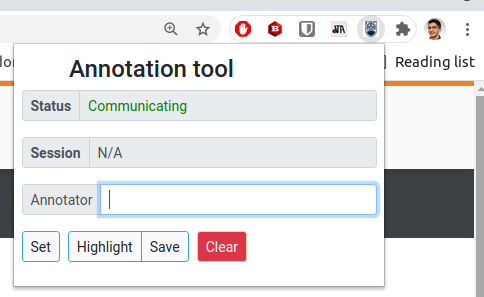
\includegraphics[width=.45\textwidth]{appendix/cp4/fig/annotation-tool.png} \smallskip
\end{center}

3. Open the links shown on a task in new tabs \smallskip

4. Read the content of each link and write a small answer (less than 250 words) on how to complete the task. \smallskip

5. Once you wrote your answer, revisit each link and click `highlight' on the extension menu \smallskip

6. After that, hovering over a sentence will display it in blue. \smallskip


7. Click on the sentence to highlight it. Highlighted sentences are shown in orange, for example: \smallskip


\begin{center}
    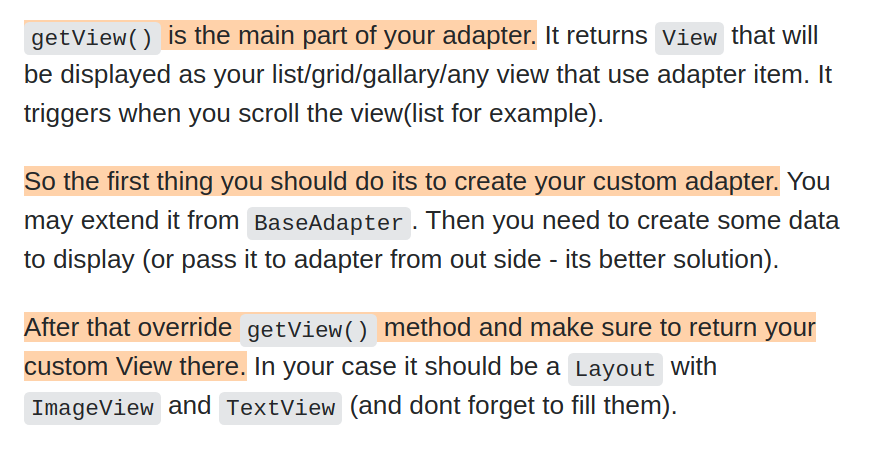
\includegraphics[width=.65\textwidth]{appendix/cp4/fig/highlight-orange.png} \smallskip
\end{center}


8. Once you have finished highlighting, click the save button on the extension menu and a copy of your highlights will be saved.

\end{scriptsize}
\end{mdframed}
\caption{Instructions about the annotation tool}
\end{figure}

